\pdfoutput=1
\documentclass[preview]{standalone}

\usepackage[utf8]{inputenc}
\usepackage{lmodern}
\usepackage[T1]{fontenc}

\usepackage{verbatim}
\usepackage{graphicx}
	\DeclareGraphicsRule{*}{mps}{*}{}
\usepackage{xcolor}

\usepackage{tikz}
	\usetikzlibrary{calc}
	\usetikzlibrary{arrows}
	\usetikzlibrary{backgrounds}
	\usetikzlibrary{decorations.pathmorphing}
	\usetikzlibrary{shapes.geometric}
	\tikzset{>=latex'}

\usepackage{amsmath}
\usepackage{amssymb}
\usepackage{dsfont}
\usepackage{nicefrac}
\usepackage{mathrsfs}
\usepackage[Euler]{upgreek}
\usepackage[nointegrals]{wasysym}
\usepackage{booktabs}
\usepackage{float}

\begin{document}

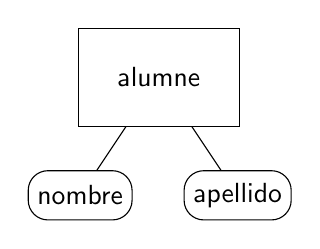
\begin{tikzpicture}[font=\sffamily]
	\node[draw,inner sep=5mm] (alumne) at (1,0) {alumne};
	\node[draw,rounded corners=2.5mm,minimum height=6.25mm] (nombre) at (0,-1.5) {nombre};
	\node[draw,rounded corners=2.5mm,minimum height=6.25mm] (apellido) at (2,-1.5) {apellido};
	\draw (alumne)--(nombre);
	\draw (alumne)--(apellido);
\end{tikzpicture}

\end{document}
